\section{Functional Requirements}
    \subsection{Data4Help}
        \subsubsection{Individual registration/log in}
            Every user who wants to use \emph{D4H} should be registered to the application System. After registration the user has to sign in, in order to collect data.\\

            \begin{table}[H]
            
            	\centering
                
                \begin{tabular}{|p{3cm}|p{8.2cm}|}
                    \hline
                    \textbf{Actors} & \begin{itemize}
                                          \item Visitor
                                          \item Individual
                                      \end{itemize}\\
                    \hline
                    \textbf{Goals} & \\ 
                     \hline
                    \textbf{Entry Condition} & The user who wants to register must have a smart-watch or fitness-band\\
                     \hline
                    \textbf{Events Flow} & \begin{enumerate}
                                                \item The Visitor accesses the application log in page.
                                                \item The Visitor clicks on the ``\emph{Register}" button and then fills in all the mandatory information (name, surname, fiscal code, password and email) in order to create an Individual account.
                                                \item The D4H System registers the user and sends back a confirmation email.
                                                \item The Visitor has to associate his smart-watch or fitness-band to the account.
                                                \item The Visitor becomes an Individual, inserting its email and password in the log in page.
                                            \end{enumerate}\\
                     \hline
                    \textbf{Exit Condition} & Now the user has his personal account.\\
                     \hline
                    \textbf{Exception} & The Registered user is not able to sign in the System because the ID (fiscal code for individual) or password are wrong or if he did not confirmed his email. In these situations, the system will show the user an error message.\\
                     \hline
                \end{tabular}  
            \end{table}
            
            \begin{figure}[H]
                \centering
                \makebox[\textwidth][c]{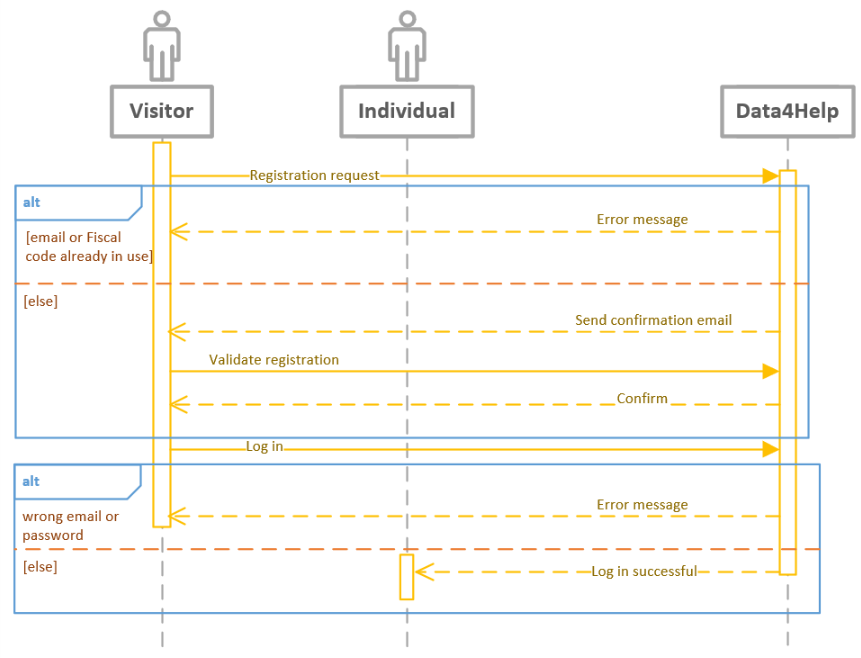
\includegraphics[scale=0.70]{pictures/IndividualRegistrationSequenceDiagram.png}}
                \caption{Sequence diagram representing the registration/log in phase of an Individual.}
                \label{fig:seq-diagram1}
            \end{figure}
        
        \subsubsection{Third-party registration and log in}
            In order to have access to the functionalities of the application, Visitors have to register to the service as Third-parties. After that, they will be able to log into the application using their email and password and to perform their researches.
            
            \begin{table}[H]
            	\centering
                \begin{tabular}{|p{3cm}|p{8.2cm}|}
                    \hline
                    \textbf{Actors} &  \begin{itemize}
                        \item Visitor
                        \item Third-party
                    \end{itemize} \\
                     \hline
                    \textbf{Goals} & G1.1, G1.2, G1.3, G1.4 \\ 
                     \hline
                    \textbf{Entry Condition} & There is no entry condition. \\
                     \hline
                    \textbf{Events Flow} & \begin{enumerate}
                        \item The Visitor accesses the registration page.
                        \item The Visitor clicks on the ``\emph{Register}" button and then fills in all the necessary information useful to be recognised as Third-party (company name, VAT code, email and password).
                        \item \emph{Data4Help} creates a new account and sends a confirmation email to the just registered Third-party.
                        \item The newly registered Third-party can now log into the application using the email and password previously provided, so to have access to the available features.
                    \end{enumerate} \\
                     \hline
                    \textbf{Exit Condition} & The Third-party is registered and able to log into \emph{Data4Help}. \\
                     \hline
                    \textbf{Exception} & The Visitor is not able to register because the email or the VAT code                      are already in use. \newline
                                         A registered Third-Party is not able to log in because the email or password inserted are wrong or the email has not been confirmed. \newline
                                         These exceptions will be handled by the system sending an error message. \\
                     \hline
                \end{tabular}  
            \end{table}
            
            \begin{figure}[H]
                \centering
                \makebox[\textwidth][c]{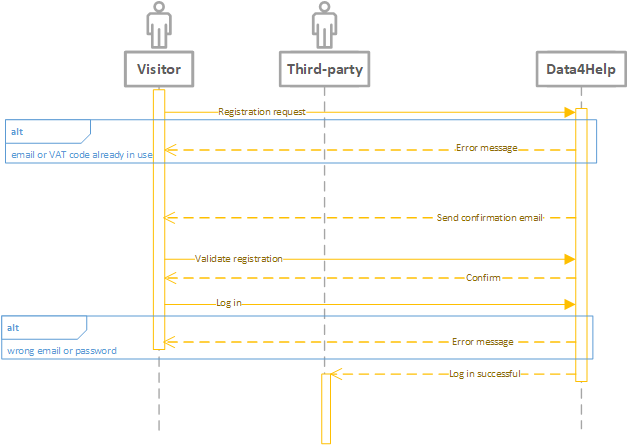
\includegraphics[scale=0.73]{pictures/RegistrationSequenceDiagram.png}}
                \caption{Sequence diagram representing the registration/log in phase of a Third-party.}
                \label{fig:seq-diagram2}
            \end{figure}
            
            
        \subsubsection{Single user data request and subscription}
        %gian    
            Third-parties can perform a request to Data4Help for a specific users by specifying his/her fiscal code. Data4Help forwards it to the User that can accept or refuse it. Then, in case of positive answer, Data4Help sends the user's health data to the applicant. If it is not, it sends a notification to the third-party informing it about the refuse.

            \begin{table}[H]
            	\centering
                
                \begin{tabular}{|p{3cm}|p{8.2cm}|}
                    \hline
                    \textbf{Actors} &  \begin{itemize}
                                            \item Third-party
                                            \item Individual
                                        \end{itemize}\\
                     \hline
                    \textbf{Goals} & \ref{goal1 : individual monitoring}\\ 
                     \hline
                    \textbf{Entry Condition} & Third-party has to be registered to Data4Help.\\
                     \hline
                    \textbf{Events Flow} & \begin{enumerate}
                                                \item The Third-Party selects "search by Fiscal Code" and it inserts the Fiscal Code of the desired person.
                                                \item The System receives the request.
                                                \item The System looks for the user connected to the Fiscal Code requested and forwards him/her the request.
                                                \item The User receives the request with the name of who is requesting his/her data.
                                                 \item The User can accept or refuse the request. By accepting it, he/she allows the System to send all his/her health data to the applicant.
                                            \end{enumerate}\\
                     \hline
                    \textbf{Exit Condition} & The Third-party has the user's health data and receive updates of them periodically. \\
                     \hline
                    \textbf{Exception} & The Fiscal Code requested doesn't match with any registered user. In this case, the system notifies it with a pop-up in the third-party application. In addition, the user may refuse the request. Then the System send a message to the Third-party notifying it about that. \\
                     \hline
                \end{tabular}  
            \end{table} 
            
            
        \subsubsection{Single User data unsubscription}
            After a successful subscription request, both Third-party or Individual can make a request in order to break the subscription to the specified data.

            \begin{table}[H]
            	\centering
                
                \begin{tabular}{|p{3cm}|p{8.2cm}|}
                    \hline
                    \textbf{Actors} &  \begin{itemize}
                                            \item Third-party
                                            \item Individual
                                        \end{itemize}\\
                     \hline
                    \textbf{Goals} & \ref{goal1: individual privacy}\\ 
                     \hline
                    \textbf{Entry Condition} & Third-party is logged in and has previously subscribed to the Individual's data.\\
                     \hline
                    \textbf{Events Flow} & \begin{enumerate}
                                                \item The Third-Party or Individual access to the subscription page and select the subscription to be cancelled.
                                                \item The Third-party or the Individual presses ``\emph{Unsubscribe}" button.
                                                \item The system deletes the Third-party subscription and sends an email to both Third-party and Individual.
                                            \end{enumerate}\\
                     \hline
                    \textbf{Exit Condition} & The Third-party is not subscribed anymore, but it has access to the previously received data. \\
                     \hline
                    \textbf{Exception} & There are no exceptions. \\
                     \hline
                \end{tabular}  
            \end{table} 
            
            \begin{figure}[H]
                \centering
                \makebox[\textwidth][c]{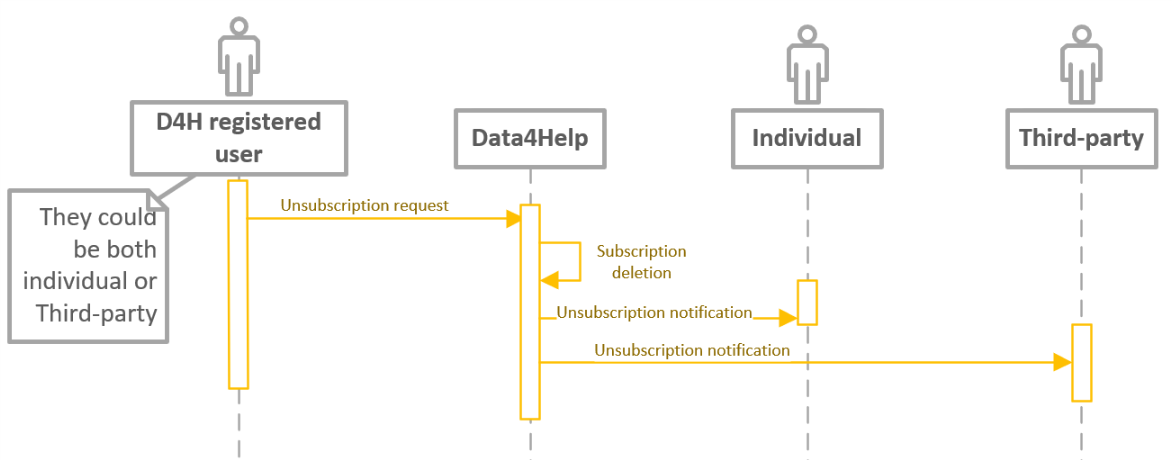
\includegraphics[scale=0.60]{pictures/IndividualRequestUnsubscriptionSequenceDiagram.png}}
                \caption{Sequence diagram representing the Unsubscription process for an individual data subscription.}
                \label{fig:Individual-request-unsubscription-process-sequence-diagram}
            \end{figure}
            
        \subsubsection{Aggregated user data request and subscription}
            Third-parties can perform group queries, asking for data coming from several Individuals that are within certain parameters specified by them (geographical areas, age, genre, time of the day). These requests are evaluated directly by D4H, that sends back the requested data only if the number of Individuals involved in the research is greater than 1000. If this is not the case, D4H sends an error message to the Third-party.

            \begin{table}[H]
            	\centering
                \begin{tabular}{|p{3cm}|p{8.2cm}|}
                    \hline
                    \textbf{Actors} &  \begin{itemize}
                        \item Third-party
                    \end{itemize} \\
                     \hline
                    \textbf{Goals} & \ref{goal1 : monitoring}, \ref{goal1 : group monitoring}\\ 
                     \hline
                    \textbf{Entry Condition} & The Third-party is logged in. \\
                     \hline
                    \textbf{Events Flow} & \begin{enumerate}
                        \item The Third-party clicks on the ``\emph{Aggregated data research}" button.
                        \item The Third-party inserts the parameters of interest.
                        \item The Third-party decides whether it wants to subscribe to this particular research by checking the specific box or not, then clicks on the ``\emph{Search}" button to have D4H perform the query.
                        \item \emph{Data4Help} does the research and evaluates the results.
                        \item D4H sends back the result to the Third-party.
                    \end{enumerate} \\
                     \hline
                    \textbf{Exit Condition} & The Third-party receives the requested information. \\
                     \hline
                    \textbf{Exception} & The number of Individuals involved in the query is lower                        than 1000, therefore D4H sends an error message back to the                      Third-party. \\
                     \hline
                \end{tabular}  
            \end{table}
            
            \begin{figure}[H]
                \centering
                \makebox[\textwidth][c]{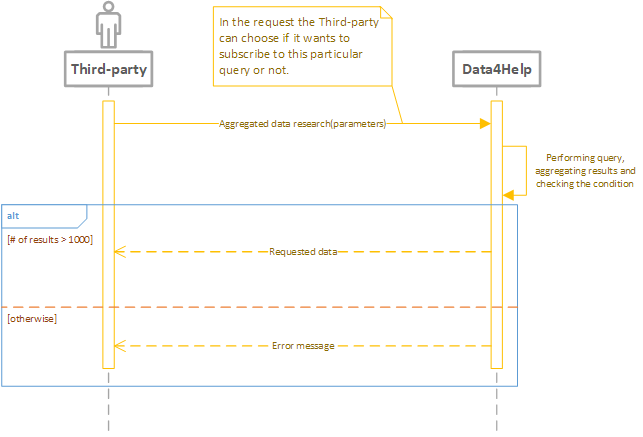
\includegraphics[scale=0.73]{pictures/Sequence2.png}}
                \caption{Sequence diagram representing the group requests performed by the Third-party.}
                \label{fig:Group-request-sequence-diagram}
            \end{figure}
            
        \subsubsection{Aggregated user data unsubscription}
        After a successful subscription to a group search, a Third-party can cancel it at any time if it does not wish to receive any further update. He will, however, still have access to the data collected until that point.
        
            \begin{table}[H]
            	\centering
                \begin{tabular}{|p{3cm}|p{8.2cm}|}
                    \hline
                    \textbf{Actors} &  \begin{itemize}
                        \item Third-party
                    \end{itemize} \\
                     \hline
                    \textbf{Goals} & \\ 
                     \hline
                    \textbf{Entry Condition} & The Third-party is logged in and has previously subscribed to a group search. \\
                     \hline
                    \textbf{Events Flow} & \begin{enumerate}
                        \item The Third-Party accesses to the subscription page and selects the subscription to be cancelled.
                        \item The Third-party presses the ``\emph{Unsubscribe}" button.
                        \item The system deletes the Third-party subscription and sends an email to it for confirmation.
                    \end{enumerate} \\
                     \hline
                    \textbf{Exit Condition} & The Third-party is not subscribed anymore, but it has access to the previously received data. \\
                     \hline
                    \textbf{Exception} & There are no exceptions. \\
                     \hline
                \end{tabular}  
            \end{table}        
        
            \begin{figure}[H]
                \centering
                \makebox[\textwidth][c]{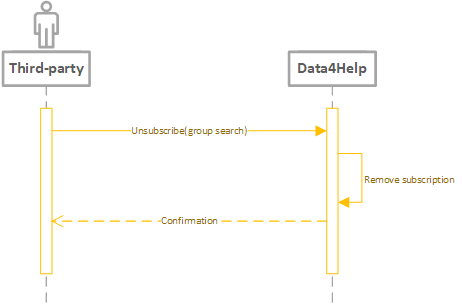
\includegraphics[scale=0.73]{pictures/Sequence3.png}}
                \caption{Sequence diagram representing the unsubscription from a group search by a Third-party.}
                \label{fig:Group-request-unsubscription-process-sequence-diagram}
            \end{figure}
        
        \subsubsection{Data Collection}
            
            Upon registration, Individuals allows the D4H system to collect their data and store them. To gather data, it's mandatory to have a device (smart-watch or fitness-band). 
            
            \begin{table}[H]
            	\centering
                
                \begin{tabular}{|p{3cm}|p{8.2cm}|}
                    \hline
                    \textbf{Actors} & \begin{itemize}
                        \item Individual
                    \end{itemize} \\
                     \hline
                    \textbf{Goals} & \\ 
                     \hline
                    \textbf{Entry Condition} & The user is correctly registered and logged into the D4H system.\\
                     \hline
                    \textbf{Events Flow} & \begin{enumerate}
                                                \item Smart-watches or fitness-band samples specific data.
                                                \item This device sends acquired data to D4H system.
                                                \item The system stores data and makes them visible to the owner Individual.
                                            \end{enumerate}\\
                     \hline
                    \textbf{Exit Condition} & The individual has personal data storage in his D4H account.\\
                     \hline
                    \textbf{Exception} & If the associate device (smart-watch or fitness-band) does not work or does not send data anymore the exception will be handled by the system by sending an error message. \\
                     \hline
                \end{tabular}  
            \end{table} 
            
            \begin{figure}[H]
                \centering
                \makebox[\textwidth][c]{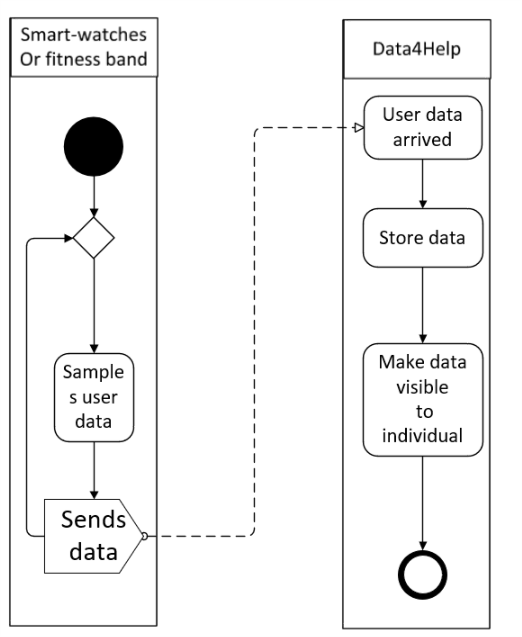
\includegraphics[scale=0.60]{pictures/DataStorageActivityDiagram.png}}
                \caption{Activity diagram representing data storage process.}
                \label{fig:Data-storage-activity-diagram}
            \end{figure}
            
    \subsection{Automated SOS}
            
        \subsubsection{Subscription Request}
            
            Every Individual, user registered to D4H, can ask for subscription to Automated SOS service, but only Elderly people will be allowed to use it.
            
            \begin{table}[H]
            	\centering
                
                \begin{tabular}{|p{3cm}|p{8.2cm}|}
                    \hline
                    \textbf{Actors} & \begin{itemize}
                        \item Individual
                    \end{itemize} \\
                     \hline
                    \textbf{Goals} & \\ 
                     \hline
                    \textbf{Entry Condition} & The user has a D4H account. \\
                     \hline
                    \textbf{Events Flow} & \begin{enumerate}
                                               \item The Individual presses on
                                               ``\emph{AutomatedSOS service}", in order to make a new subscription request.
                                               \item The ASOS System checks if the petitioner is at least 65 years old.
                                               \item If verified, the user gets subscribed.
                                           \end{enumerate}\\
                     \hline
                    \textbf{Exit Condition} & The Individual is now subscribed to Automated SOS service.\\
                     \hline
                    \textbf{Exception} & If the petitioner is less then 65 years old, the system handles the exception, sending him an error message. \\
                     \hline
                \end{tabular}  
            \end{table} 
            
            \begin{figure}[H]
                \centering
                \makebox[\textwidth][c]{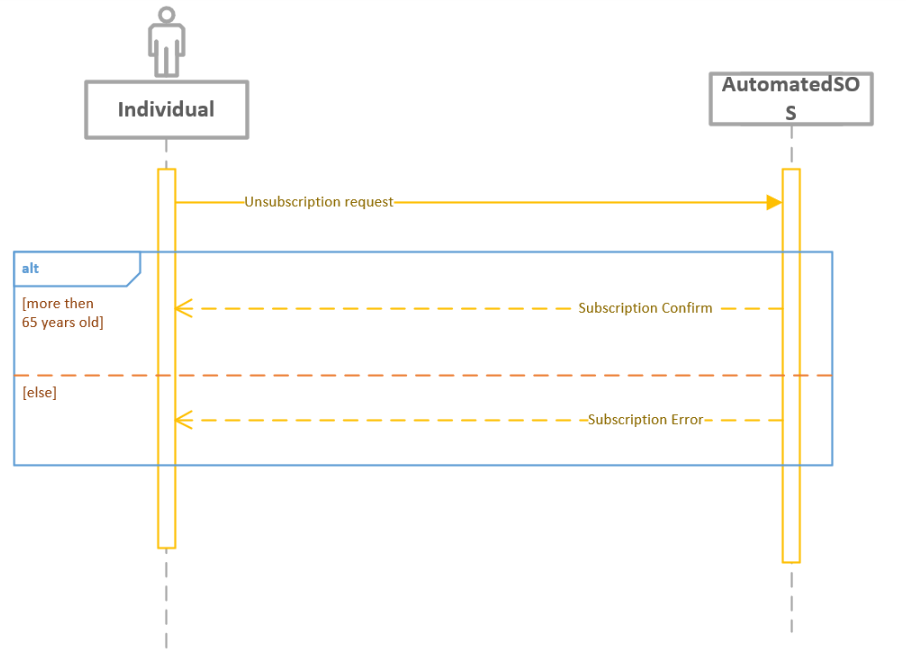
\includegraphics[scale=0.70]{pictures/ASOSubscriptionRequest.png}}
                \caption{Sequence diagram representing the subscription request for ASOS service.}
                \label{fig:ASOS-seq-diagram1}
            \end{figure}
            
        \subsubsection{Ambulance dispatching}
                Whenever the system receives a value that goes beyond the critical threshold, ASOS contacts the ambulance service, asking for assistance.
                
            \begin{table}[H]
            	\centering
                
                \begin{tabular}{|p{3cm}|p{8.2cm}|}
                    \hline
                    \textbf{Actors} & \begin{itemize}
                        \item Elderly person
                        \item Ambulance service
                    \end{itemize} \\
                     \hline
                    \textbf{Goals} & \\ 
                     \hline
                    \textbf{Entry Condition} & The user has an ASOS account and is logged in. \\
                     \hline
                    \textbf{Events Flow} & \begin{enumerate}
                                               \item D4H collects through the connected device the Elderly person's data.
                                               \item ASOS checks if the values are under the critical threshold.
                                               \item If so, ASOS contacts the ambulance service, giving the location of the Elderly person gathered with the last measurement. Otherwise, it does nothing.
                                               \item The ambulance service sends an ambulance to the Elderly person location.
                                           \end{enumerate} \\
                     \hline
                    \textbf{Exit Condition} & The ambulance service has been warned and an ambulance in arriving at the Elderly person place. \\
                     \hline
                    \textbf{Exception} & There are no exceptions. \\
                     \hline
                \end{tabular}  
            \end{table}                 
            
            \begin{figure}[H]
                \centering
                \makebox[\textwidth][c]{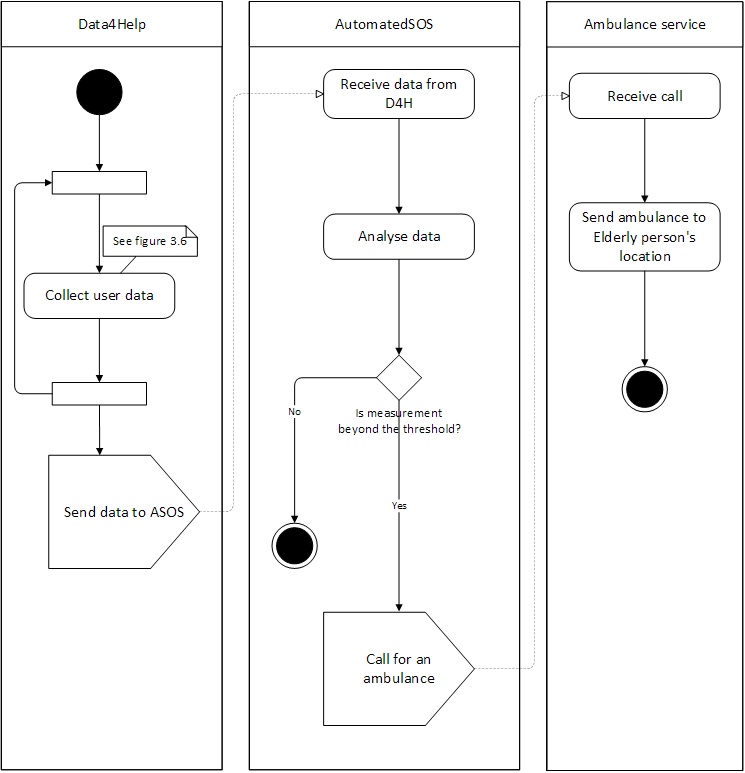
\includegraphics[scale=0.6150]{pictures/Activity1.png}}
                \caption{Activity diagram representing the call for an ambulance that ASOS performs when a critical measurement is collected by D4H.}
                \label{fig:ASOS-activity-diagram1}
            \end{figure}
            
    \subsection{Track4Run}
        
        \subsubsection{Organiser registration and log in}
            Any Organiser needs to register to T4R before being able to organise and publish races. This account is in no way dependant to D4H and Organisers do not need to be registered to D4H too. Therefore, if they are already registered to D4H as Third-parties, they still need a new account, but can use the same information provided for D4H. 
            
            \begin{table}[H]
            	\centering
                
                \begin{tabular}{|p{3cm}|p{8.2cm}|}
                    \hline
                    \textbf{Actors} & \begin{itemize}
                        \item Visitor
                        \item Organiser
                    \end{itemize} \\
                     \hline
                    \textbf{Goals} & \\ 
                     \hline
                    \textbf{Entry Condition} & There is no entry condition. \\
                     \hline
                    \textbf{Events Flow} & \begin{enumerate}
                                               \item The Visitor accesses the application log in page.
                                               \item The Visitor clicks on the ``\emph{Register}" button and then fills in all the mandatory information (company name, VAT code, email and password).
                                               \item T4R creates a new account and sends a confirmation email to the just registered Organiser.
                                               \item The newly registered Organiser can now log into the application using the email and password previously provided, so to have access to the available features.
                                           \end{enumerate} \\
                     \hline
                    \textbf{Exit Condition} & The Organiser is registered and able to log into                                \emph{Track4Run}. \\
                     \hline
                    \textbf{Exception} & The Visitor is not able to register because the email or the VAT code                      are already in use. \newline
                                         A registered Organiser is not able to log in because the email or password inserted are wrong or the email has not been confirmed. \newline
                                         These exception will be handled by the system sending an error message. \\
                                         \hline
                \end{tabular}  
            \end{table}
            
            \begin{figure}[H]
                \centering
                \makebox[\textwidth][c]{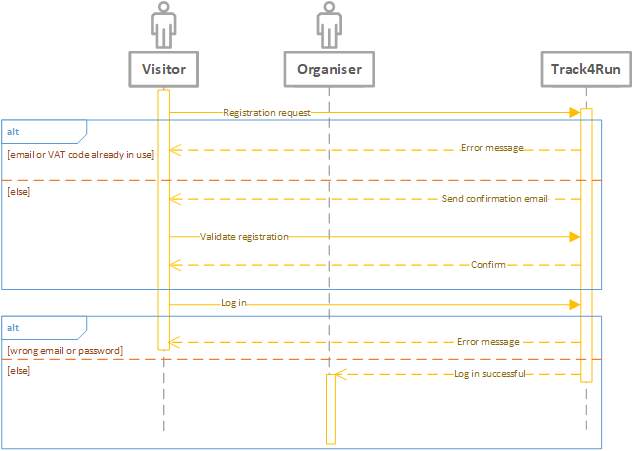
\includegraphics[scale=0.73]{pictures/Sequence4.png}}
                \caption{Sequence diagram representing the registration of an Organiser to T4R.}
                \label{fig:Organiser-registration-sequence-diagram}
            \end{figure}
            
        \subsubsection{Run organisation}
            
            The T4R system allows registered organisers to organise a run. They have to specify the time and the place, but it is not possible to add if there is another, already stored, race in the same place and at the same time. Different runs at the same time but different place are allowed.
            
            \begin{table}[H]
            	\centering
                
                \begin{tabular}{|p{3cm}|p{8.2cm}|}
                    \hline
                    \textbf{Actors} & \begin{itemize}
                        \item Organiser
                    \end{itemize} \\
                     \hline
                    \textbf{Goals} & \\ 
                     \hline
                    \textbf{Entry Condition} & Organiser must have an organiser account in T4R system.\\
                     \hline
                    \textbf{Events Flow} & \begin{enumerate}
                                                \item The Organiser presses on ``\emph{New Run}" button.
                                                \item The Organiser specifies date, time, place and the maximum number of participants.
                                                \item The system creates this new run, stores it and sends a notification email to the Organiser.
                                            \end{enumerate}\\
                     \hline
                    \textbf{Exit Condition} & A new race has been created.\\
                     \hline
                    \textbf{Exception} & If there is another stored race with the same data, time and place, the system                       handles the exception, showing an error message to the organiser. \\
                     \hline
                \end{tabular}  
            \end{table} 
            
            \begin{figure}[H]
                \centering
                \makebox[\textwidth][c]{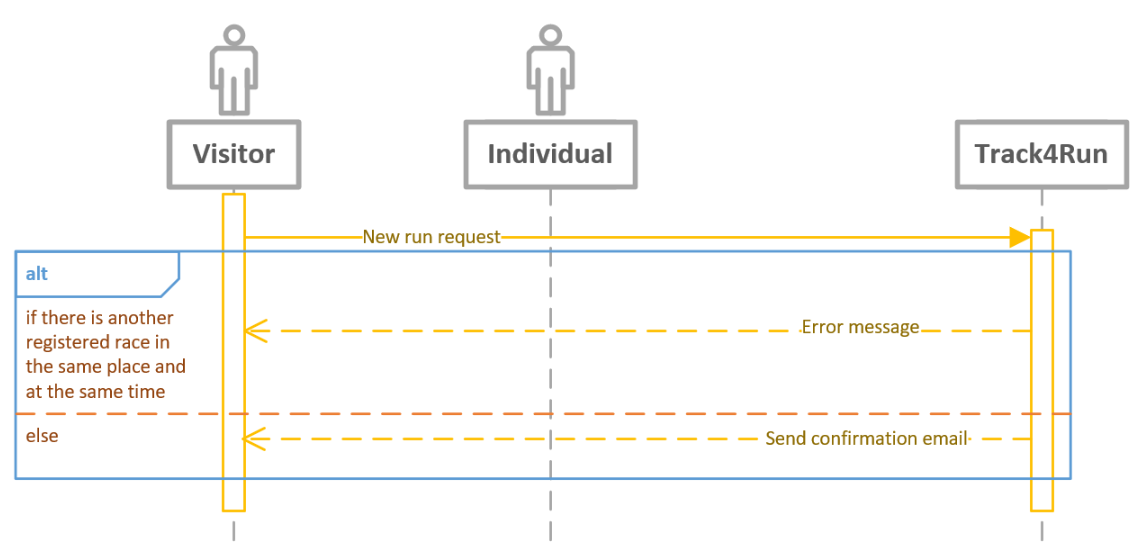
\includegraphics[scale=0.60]{pictures/OrganizationRunSequenceDiagram.png}}
                \caption{Sequence diagram representing the request in order to create a new run.}
                \label{fig:T4R-run-organization}
            \end{figure}
            
        \subsubsection{Enrolment to a run}
            Any Participant can log into T4H using his D4H (Individual) account. After doing that, he/she will be able to see all available runs and to enrol to them. The races can be filtered by time and zone, as to simplify the research.
            
            \begin{table}[H]
            	\centering
                
                \begin{tabular}{|p{3cm}|p{8.2cm}|}
                    \hline
                    \textbf{Actors} & \begin{itemize}
                        \item Participant
                    \end{itemize} \\
                     \hline
                    \textbf{Goals} & \\ 
                     \hline
                    \textbf{Entry Condition} & The Participant is logged into T4R, using his D4H Individual account. \\
                     \hline
                    \textbf{Events Flow} & \begin{enumerate}
                                                \item The participant clicks on the ``\emph{Show available races}" button.
                                                \item The Participant looks through the available races, eventually filtering them to ease the search, and selects one of them.
                                                \item The Participant presses on ``\emph{Enrol}" button.
                                                \item T4R sends a confirmation mail to the Participant.
                                            \end{enumerate}\\
                     \hline
                    \textbf{Exit Condition} & The Participant is enrolled to the selected race.\\
                     \hline
                    \textbf{Exception} & If the Participant is already enrolled to another race at the same time, an                          error message is sent to him/her. \newline
                                         If the race has reached the maximum number of subscriptions, an error message is sent to the Participant. \\
                     \hline
                \end{tabular}  
            \end{table}            
            
            \begin{figure}[H]
                \centering
                \makebox[\textwidth][c]{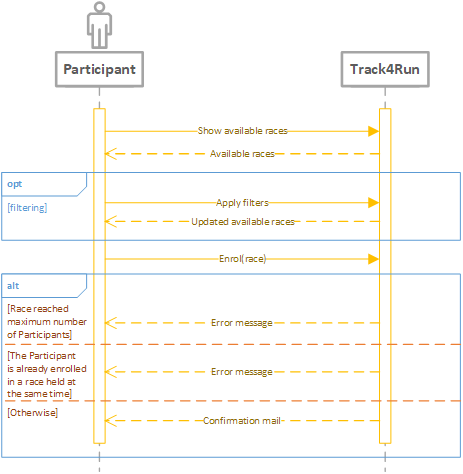
\includegraphics[scale=0.97]{pictures/modelT4R_ParticipantEnrollment.png}}
                \caption{Sequence diagram representing the enrolment to a run of a Participant.}
                \label{fig:T4R-participant-enrolment}
            \end{figure}
            
        \subsubsection{Participant tracking}
            
            Every Visitor, registered or not, is able to track participants on a map during the race and, if there is more then one run at the same time, they can choose which run to watch. To provide this service, the system interacts with Google Maps.
            
            \begin{table}[H]
            	\centering
                
                \begin{tabular}{|p{3cm}|p{8.2cm}|}
                    \hline
                    \textbf{Actors} & \begin{itemize}
                                            \item Visitor
                                            \item Map service
                                        \end{itemize} \\
                     \hline
                    \textbf{Goals} & \\ 
                     \hline
                    \textbf{Entry Condition} & There is no entry condition \\
                     \hline
                    \textbf{Events Flow} & \begin{enumerate}
                                                \item The Visitor launches the application.
                                                \item They press on the ``\emph{Track runners}" button.
                                                \item The system shows the list of current runs.
                                                \item The Visitor selects the run of interest.
                                                \item The system asks for map and runners positions to the map service.
                                                \item The map service sends to the system map and runners location.
                                                \item The system shows the map with all runners current position.
                                                \item If the Visitor follows the run until the end, T4R shows to him the rank.
                                            \end{enumerate} \\
                     \hline
                    \textbf{Exit Condition} & Visitors are now able to see runners on a map (and the rank if the stay until the race is over). \\
                     \hline
                    \textbf{Exception} & If there are no runs in that moment, the system handles the exception, showing a notification message. \\
                     \hline
                \end{tabular}  
            \end{table}
            
            \begin{figure}[H]
                \centering
                \makebox[\textwidth][c]{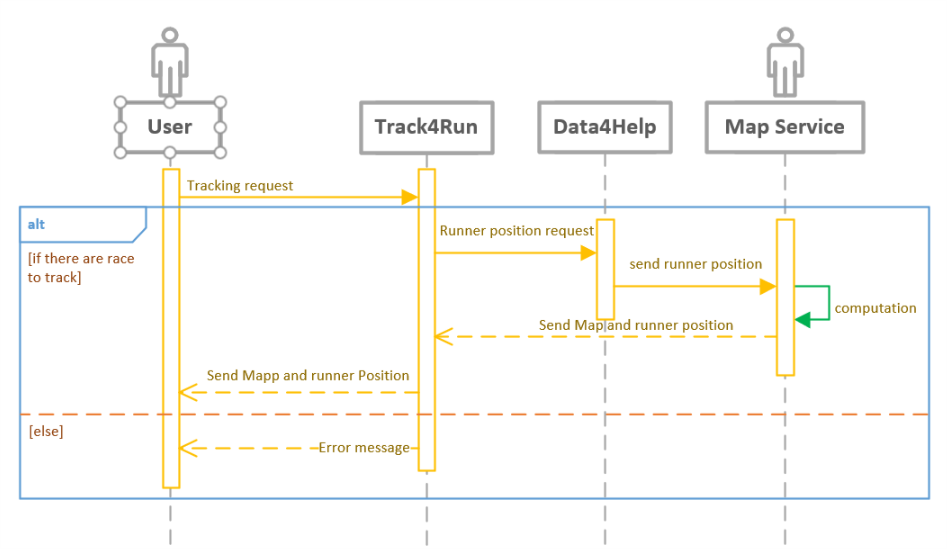
\includegraphics[scale=0.70]{pictures/TrackingSequenceDiagram.png}}
                \caption{Sequence diagram representing the request in order to see participant position on a map during the run.}
                \label{fig:T4R-runner-tracking}
            \end{figure}
            
        \subsubsection{Rank history}
            Participants and Organisers are able to see the rank for all past races they have took part in or organised, respectively. Since the procedure to access the rank history is the same for the two actors, only one use case is provided.

            \begin{table}[H]
            	\centering
                
                \begin{tabular}{|p{3cm}|p{8.2cm}|}
                    \hline
                    \textbf{Actors} & \begin{itemize}
                                            \item Participant / Organiser
                                        \end{itemize} \\
                     \hline
                    \textbf{Goals} & \\ 
                     \hline
                    \textbf{Entry Condition} & The Participant has took part in / The Organiser has organised at least                              one run and is logged in. \\
                     \hline
                    \textbf{Events Flow} & \begin{enumerate}
                                                \item The Participant / Organiser clicks on the ``\emph{Runs history}" tab.
                                                \item The Participant / Organiser selects the run of which he/she wishes to see the rank.
                                                \item T4R shows the rank to the Participant / Organiser.
                                            \end{enumerate} \\
                     \hline
                    \textbf{Exit Condition} & The Participant / Organiser is able to see the rank of the selected race                             he/she has took part in / organised. \\
                     \hline
                    \textbf{Exception} & If the Participant has not took part in any run, an error                       message is sent to him/her. \newline
                                         If the Organiser has not organised any run, an error message is sent to him/her. \\
                     \hline
                \end{tabular}  
            \end{table}
            
            \begin{figure}[H]
                \centering
                \makebox[\textwidth][c]{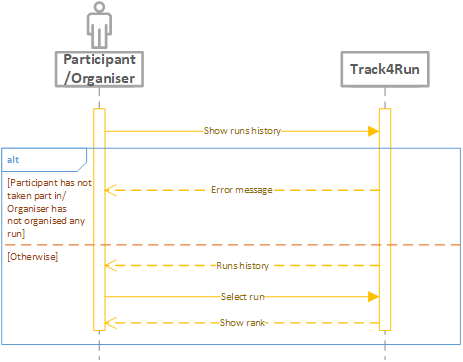
\includegraphics[scale=0.97]{pictures/modelT4R_RankHistory.png}}
                \caption{Sequence diagram representing request for the rank of a run.}
                \label{fig:T4R-rank-history}
            \end{figure}